% TODO there is too much information in this part. simply repeating slides is probably not such a good idea. one compromise could be to eliminate all discussion slides and rather present this information only in form of tables

\subsection{Recap: Runtime Variability}
\againframe<2>{GraphWithGlobalVariables}
\againframe<2>{SPLwithPreferenceDialogsCommandLineOptionsConfigurationFiles}
\againframe<3>{SPLwithImmutableGlobalVariables}
\againframe<3>{PrinciplesAndProblemsOfRuntimeVariability}

\subsection{Recap: Clone-and-Own}
% TODO avoid cloning the content of this slide (copied from multiple slides)
\begin{frame}{\myframetitle}
	\begin{fancycolumns}[animation=none]
		\begin{definition}{Clone-and-Own}
			\begin{itemize}
				\item New variants of a software system are created by copying and adapting an existing variant.
				\item Afterwards, cloned variants evolve independently of each other.
			\end{itemize}	
		\end{definition}	
		\vspace{3mm}		
		\begin{example}{Cloning Whole Products (Clone-and-Own)}
			~\hfill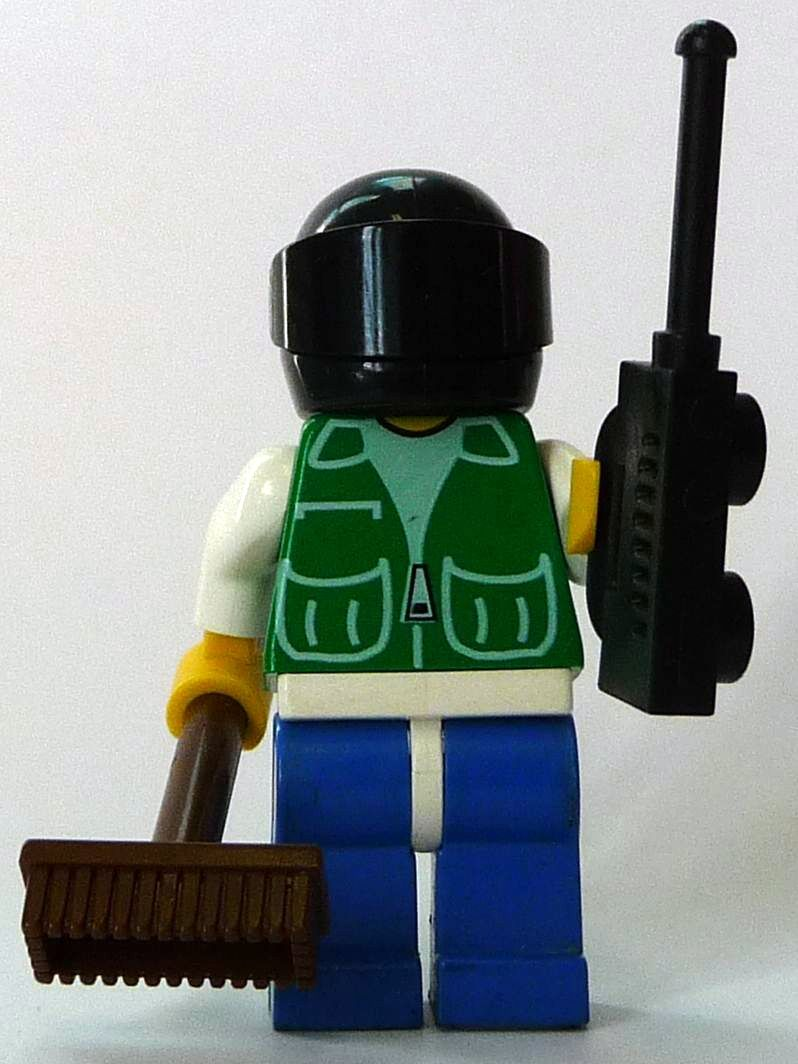
\includegraphics[width=.2\linewidth]{130}\hfill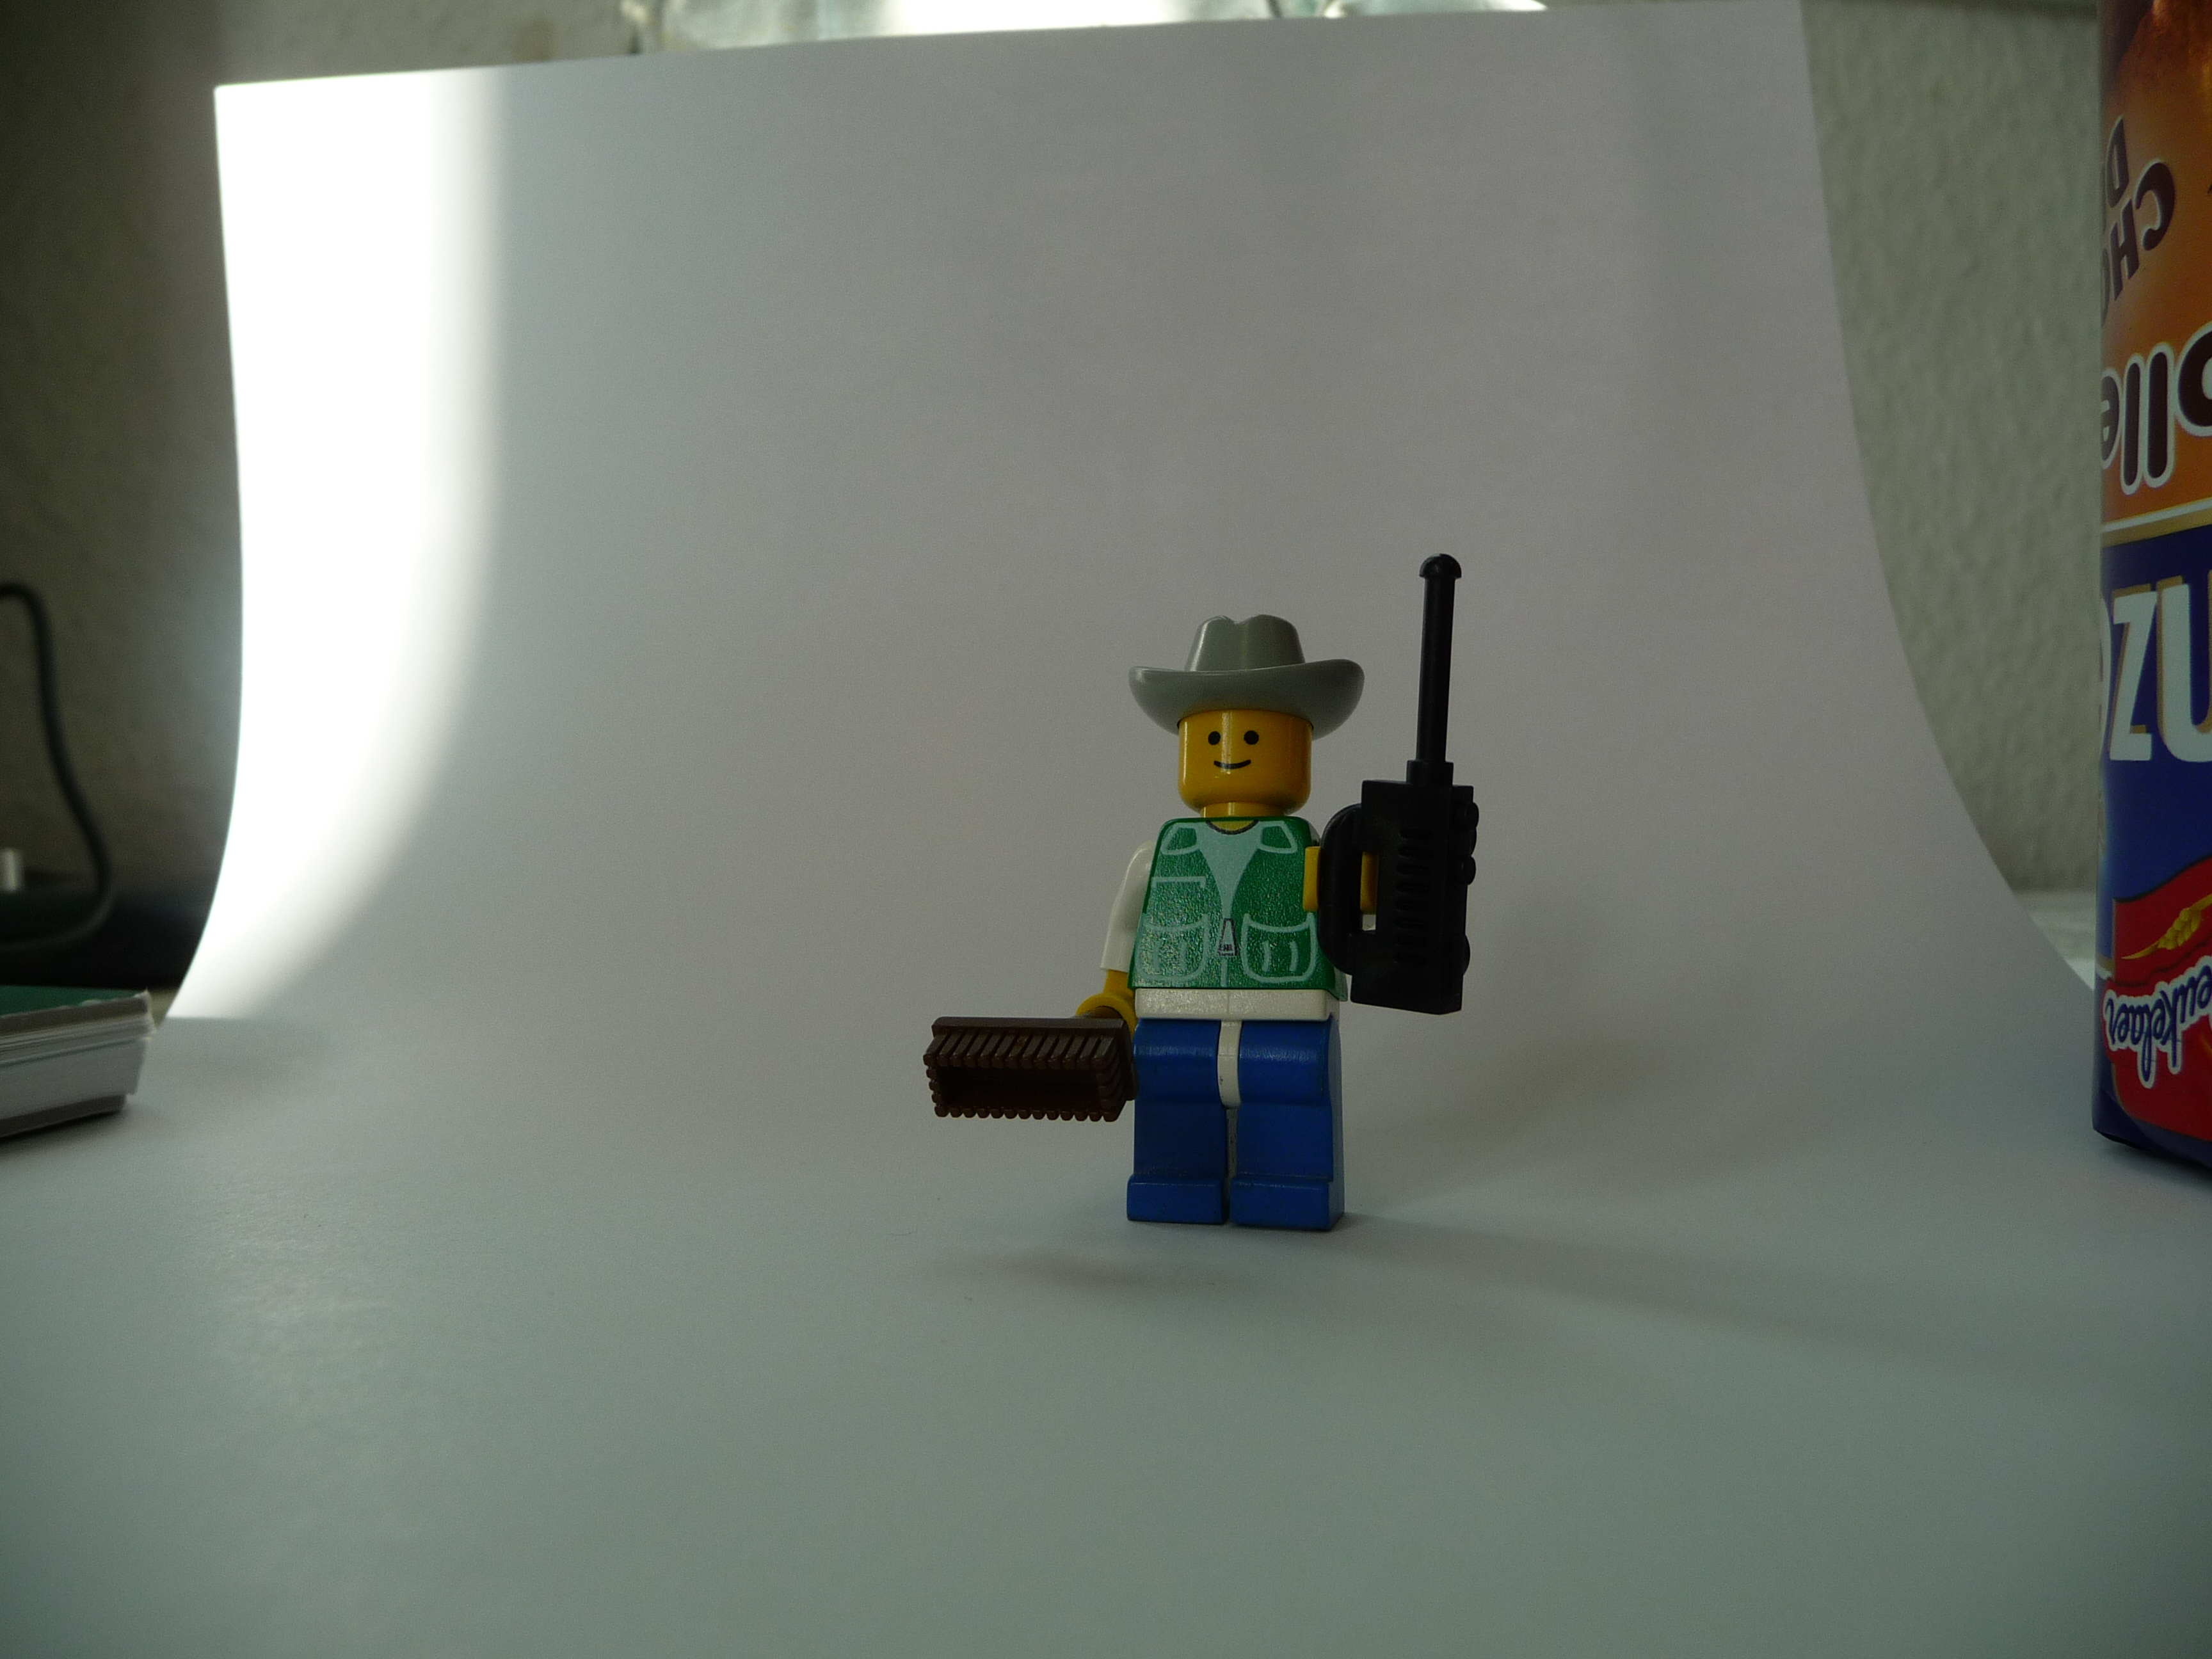
\includegraphics[width=.2\linewidth]{230}\hfill~
		\end{example}
	\nextcolumn
		\pic[width=\linewidth,page=24]{lego}
	\end{fancycolumns}
\end{frame}
\againframe<2>{SPLwithCloneAndOwn}

\subsection{Recap: Conditional Compilation}

\subsubsection*{Build Systems}
\againframe<3>{SPLwithBuildSystems}
\againframe<3>{DiscussionOfBuildSystems}

\subsubsection*{Preprocessors}
\againframe<8>{SPLwithPreprocessors}
\againframe<3>{DiscussionOfPreprocessors}

\subsection{Recap: Modular Features}

\subsubsection*{Components}
\againframe<2>{SPLwithComponents}

\subsubsection*{Services}
\againframe<4>{SPLwithServices}

\subsubsection*{Frameworks with Plug-Ins}
\againframe<5>{SPLwithPlugIns}
\againframe<3>{ChallengesOfPlugins}

\subsection{Recap: Languages for Features}

\subsubsection*{Feature-Oriented Programming}
\againframe<3>{SPLwithFeatureModules}
\againframe<2>{DiscussionOfFeatureModules}

\subsubsection*{Aspect-Oriented Programming}
\againframe<2>{SPLwithAspects}
\againframe<3>{DiscussionOfAspects}

\subsection{Comparison of Implementation Techniques}
\begin{frame}[label=ComparisonOfImplementationTechniques,fragile]{\myframetitle}
	\centering
	\renewcommand{\arraystretch}{1.2}
	\newcommand{\myexception}[1]{\tiny{}(#1)}
	\begin{tabular}{p{32mm}p{32mm}p{14mm}p{27mm}p{14mm}}
		 & Compile-Time Variability & Features & Product Generation & Feature \mbox{Traceability} \pause\\\rowcolor{gray}
		Runtime Variability & no \myexception{very limited for immutable global variables} & only fine grained & yes \mbox{\myexception{except for preference dialogs}} & no \pause\\
		Clone-and-Own & yes \linebreak\myexception{only for implemented products} & no & no \myexception{limited generation for clone-and-own with build systems} & no \pause\\\rowcolor{gray}
		\mbox{Build Systems} \mbox{\myexception{for Conditional Compilation}} & yes & only coarse grained & yes & with tool support \pause\\
		Preprocessors \mbox{\myexception{for Conditional Compilation}} & yes & only fine grained & yes & with tool support \pause\\\rowcolor{gray}
		Components/Services & yes & only coarse grained & no \linebreak\myexception{except pure exchange} & only coarse grained \pause\\
		Frameworks with Plug-Ins & yes & only coarse grained & yes & only coarse grained \pause\\\rowcolor{gray}
		Feature Modules/Aspects & yes & yes & yes & yes \pause\\
	\end{tabular}
	\begin{note}{Further Criteria}
		interfaces between features? code duplication necessary? modularization of cross-cutting concerns? \ldots
	\end{note}
\end{frame}
% TODO animate table adding only columns relevant so far https://tex.stackexchange.com/questions/345815/table-column-animation-in-beamer-not-showing-table-lines-and-notes

% TODO deep software variability? https://dl.acm.org/doi/10.1145/3442391.3442402 https://www.slideshare.net/acher/tackling-deep-software-variability-together
% TODO ACCORD? https://dl.acm.org/doi/abs/10.1145/3563835.3568737
